\documentclass{article}
\usepackage{fullpage}
\usepackage{amsmath,amssymb,amsfonts}
\usepackage{graphicx}
\usepackage{natbib}
\usepackage{xcolor}

\def\R{{\mathbb{R}}}
\def\pr{{\rm Pr}}
\def\E{{\mathbb E}}
\def\X{{\mathcal X}}
\def\Y{{\mathcal Y}}
\def\H{{\mathcal H}}
\def\G{{\mathcal G}}
\def\B{{\mathcal B}}
\def\bias{{\rm bias}}
\def\supp{{\rm supp}}
\def\yh{{\widehat{y}}}
\def\PL{{\rm PL}}
\def\sign{{\rm sign}}

\newtheorem{thm}{Theorem}
\newtheorem{lemma}[thm]{Lemma}
\newtheorem{cor}[thm]{Corollary}
\newtheorem{claim}[thm]{Claim}
\newtheorem{defn}[thm]{Definition}
\newtheorem{assump}{Assumption}
\newtheorem{open}{Open problem}
\newenvironment{proof}{\noindent {\sc Proof:}}{$\Box$ \medskip}

\newcommand{\sanjoy}[1]{{\color{red} {\bf Sanjoy:} #1}}
\newcommand{\yoav}[1]{{\color{blue} {\bf Yoav:} #1}}

\DeclareMathOperator*{\argmax}{arg\,max}

\title{Active learning using the near-neighborhoods algorithm}


\begin{document}

\maketitle

\section{Setup}

\begin{itemize}
\item {\it Underlying model of data.}

\begin{itemize}
\item Instances lie in a metric space $(\X, d)$. 
\item Label space $\Y = \{-1,+1\}$. Each $x \in \X$ is labeled according to an unknown conditional probability function $\Pr(Y|X)$, with
$$ \eta(x) = \E[Y | X=x] = \pr(Y=1|X=x) - \pr(Y=-1|X=x) = 2 \pr(Y=1|X=x) - 1 .$$
\item The {\it Bayes-optimal classifier} on $\X$ is $g^*(x) = \sign(\eta(x))$.
\end{itemize}

\item {\it Task: Finite population labeling.}

\begin{itemize}
\item We are given a finite dataset of $n$ points, and have the
  ability to query the labels of any of them. The response to the
  query $x$ is +1 or -1, chosen according the conditional probability
  function $\eta(x)$. When two or more queries are made on the
  instance $x$, the responses are chosen independently at random
  according to $\eta(x)$, in other words, the labels are not persistant. 

\item We are given parameters $0 < \gamma, \delta < 1$.
\item We want a procedure that chooses the next point, or batch of points, to query. This process will be applied repeatedly and forever. At any point the procedure can be asked to make a prediction on any point in $X$. The prediction is $\yh(x) \in \{-1,0,+1\}$. We consider the prediction correct if $\yh(x)=+1$ and $\eta(x)=+1$, if $\yh(x)=-1$ and $\eta(x)=-1$ or $\yh(x)=0$ and $|\eta(x)| < \gamma$. 
\item 
Choosing the queries indepndently at random is guaranteed to reach the correct prediction after querying each example $O(1/\gamma^2)$ times for a total of $O(|X|/\gamma^2)$ queries. Our goal is to reach convergence after much fewer queries.
\item 
Our bounds are pointwise, i.e. we say that the query complexity of the point $x$ is $q(x)$ if for any number of queries larger than $q(x)$ the prediction on $x$ is correct. The hope is that for most $x$, $q(x) \ll |X|/\gamma^2)$.
\item 
Our bounds should be a function of the advantage, as defined in the adaptive KNN paper: $p \gamma^2$
\iffalse
We would like the inferred labels $\yh(x)$ to approach the Bayes-optimal labels $g^*(x)$ as quickly as possible, ideally much faster than would occur if the query points were chosen uniformly at random.
\item Specifically, we will then be judged on the number of errors on points $x \in X$ with $|\eta(x)| > \gamma$:
$$ \sum_{x \in X} {\bf 1}(\yh(x) \neq g^*(x),\ |\eta(x)| > \gamma) .$$
The procedure is allowed to fail with probability $\delta$, to account for sampling error.
\fi
\end{itemize}

\end{itemize}

\section{Active learning algorithm}

\subsection{Some details}

\begin{enumerate}

\item {\it Sampling regions.}
The sampling is organized around a collection $\B$ of measurable subsets of $\X$. These are the atomic sets on which we assess label bias and we call them ``balls''.

\begin{enumerate}

\item[(a)] {\it Points within a ball.} For any ball $B \in \B$, let $X_B$ denote the points in $X$ that can be used to assess the bias of $B$. This is simply $X_B = X \cap B$ unless $\B$ is constructed in a way that depends on $X$ and causes certain points to be excluded.\footnote{The construction of $\B$ may or may not depend on the unlabeled points $X$, and this distinction determines which points can be considered random draws from a particular $B \in \B$. For instance, consider these two alternatives for defining $\B$:
\begin{itemize}
\item $\B$ consists of a pre-defined set of balls.
\item $\B$ consists of balls defined by pairs of points in $X$, with each $x,x' \in X$ yielding the ball $B(x,\|x-x'\|)$.
\end{itemize}
In the first case, all points $X \cap B$ are random draws from $B$. In the second case, this is also true except for the two points $x,x'$ that define the ball.}

\item[(b)] {\it Grouping balls by size.} We will group balls by the number of points that they contain: we put $B$ at {\it level} $\ell$ if
$$ \frac{n}{2^{\ell + 1}} \leq |X_B| < \frac{n}{2^\ell} .$$
Here $\ell$ ranges from $0$ (consisting of balls that contain at least half the data points) to roughly $\lg n$ (containing a single point). 

Let $\B_\ell$ consist of all balls in $\B$ that are at level $\ell$. Thus $\B_0, \B_1, \ldots$ is a partition of $\B$, with $\B_0$ consisting of very large balls and subsequent $\B_1, \B_2, \ldots$ consisting of successively smaller balls.

\item[(c)] {\it Balls used to evaluate a given point.}

For any $x \in \X$, let $\B(x) \subset \B$ denote the collection of balls that will be used in determining $x$'s label. There are many ways in which this could be set, for instance,
\begin{itemize}
\item all balls containing $x$, or
\item all balls centered at $x$.
\end{itemize}
As before, we can partition these balls by sampling-level, so that $\B_\ell(x) = \B(x) \cap \B_\ell$.

\end{enumerate}

\item {\it Bias-estimates for balls and for data points.} The active learning algorithm uses label-queries to assess the bias of balls $B \in \B$. In turn, these are used to estimate the labels of individual points.

\begin{enumerate}

\item[(a)] {\it Bias of a ball.} The bias of a ball $B \in \B$ is defined as
$$ \eta_X(B) = \mbox{average}\{\eta(x): x \in X_B \} .$$

\item[(b)] {\it Qualitative estimates of bias.} Each ball $B$ is assigned qualitative bias estimate,
$$ \yh(B) = 
\left\{
\begin{array}{cl}
+1 & \mbox{significant $+$ bias} \\
-1 & \mbox{significant $-$ bias} \\
0 & \mbox{no significant bias} \\
\bot & \mbox{not yet available}
\end{array}
\right.
$$
The option $\bot$ is used until sufficiently many points in $X_B$ have been labeled: the required number, $k$, is roughly $1/\gamma^2$ (recall that $\gamma$ is the smallest bias that needs to be detected). Once $k$ labels are available, $\yh(B)$ is set to a value in $\{-1,0,+1\}$ and remains fixed thereafter.

\item[(c)] {\it Bias guarantees.} Our bias estimates will satisfy a guarantee of the following form: with probability $1-\delta$, for all $B \in \B$, once $\yh(B)$ is set to a value in $\{-1,0,+1\}$, 
\begin{itemize}
\item $\yh(B) = +1 \implies \eta_X(B) > b_1$
\item $\yh(B) = -1 \implies \eta_X(B) < -b_1$
\item $\yh(B) = 0 \implies |\eta_X(B)| < b_2$
\end{itemize}
for some constants $0 < b_1 < b_2 < 1$.

\item[(d)] {\it Possible labels for a point.} Pick any $x$ and any level $\ell$. Once bias-estimates are available for all balls $B \in \B_\ell(x)$, the possible labels for $x$ at level $\ell$ are $\PL_\ell(x) \subset \{-1,+1\}$, defined as follows:
\begin{itemize}
\item $\PL_\ell(x)$ contains $+1$ if and only if there exists $B \in \B_\ell(x)$ with $y(B) = +1$ such that there is no $B' \in \B_\ell(x)$ with $B' \subset B$ and $y(B') = -1$.
\item $\PL_\ell(x)$ contains $-1$ is defined symmetrically.
\end{itemize}

\item[(e)] {\it The label of a point at level $\ell$.} The label of point $x$ at level $\ell$ is a value $\yh_\ell(x) \in \{-1,+1,0,!,\bot\}$. It is initially $\bot$, but once bias-estimates are available for all $B \in \B_\ell(x)$, it is set to a value in $\{-1,+1,0,!\}$ and remains fixed thereafter:
\begin{equation}
\yh_\ell(x) = 
\left\{
\begin{array}{cl}
+1 & \mbox{if $\PL_\ell(x) = \{+1\}$} \\
-1 &  \mbox{if $\PL_\ell(x) = \{-1\}$} \\
0 & \mbox{if $\PL_\ell(x) = \{\}$} \\
! & \mbox{if $\PL_\ell(x) = \{-1,+1\}$}
\end{array}
\right.
\label{eq:provisional-label}
\end{equation}
Points labeled $!$ are ``known unknowns'': they are near the decision boundary and need further investigation. Points labeled $0$ show no significant bias.

\end{enumerate}

\end{enumerate}


\begin{figure}[ht!]
\framebox{
\begin{minipage}[t]{6.4in}
\vspace{.1in}
\emph{Variables:}
\begin{itemize}
\item $Q$ (queries made so far)
\end{itemize}

\vspace{.1in}
\emph{Initialization:}
\begin{itemize}
\item Set $Q := \emptyset$ (points queried so far)
\item For each $x \in X$: choose $T_x \sim \mbox{unif}[0,1]$
\end{itemize}

\vspace{.2in}
{\bf Focused-query}($\ell, U$)

\vspace{.1in}
\begin{itemize}
\item Query region:
$$ S =  \bigcup_{x \in U} \bigcup_{B \in \B_\ell(x)} \{z \in X_B: T_z \leq \tau_\ell\} $$
\item Query the next unlabeled point in $S \setminus Q$, ordered by $T_z$ values, and add to $Q$
\end{itemize}

\vspace{.2in}
{\bf Background-query}

\vspace{.1in}
\begin{itemize}
\item Query the next unlabeled point in $X \setminus Q$, ordered by $T_z$ values, and add to $Q$
\end{itemize}
\yoav{I am not sure whether the set from which to pick the query
  should exclude $Q$: the queries that have been made o far. if a set
  consists of one point and that point has a weak bias, we need to
  sample the point several times.}
\end{minipage}}
\caption{The sampling procedures. Each point $x \in X$ has an associated value $T_x$ chosen uniformly at random from $[0,1]$. This smaller this value, the earlier this point is likely to be queried. The focused querying procedure also uses threshold $\tau_\ell = 2^{\ell+2}k/n$.} 
\label{alg:sampling}
\end{figure}


\begin{figure}[ht!]
\framebox{
  \begin{minipage}[t]{6.4in}
    \vspace{.1in}
\emph{Variables:}
\begin{itemize}
\item $U_\ell$ The set of points level $\ell$ that are ``known unknowns''
\end{itemize}

\vspace{.2in}
{\bf Active Balls}
\begin{itemize}
\item Initialize uncertainty regions at all levels:
\begin{itemize}
\item $U_0 = X$
\item $U_\ell = \emptyset$ for $\ell \geq 1$
\end{itemize}

\vspace{.1in}
\item Repeat:
\begin{itemize}
\item If there is a level $\ell \geq 0$ such that $U_\ell \neq \emptyset$:
\begin{itemize}
\item Let $\ell'$ be the smallest such level
\item {\tt Focused-query}($\ell', U_{\ell'}$)
\end{itemize}
\item {\tt Background-query}
\item Update $\yh_{\ell}$ values, $\ell \geq 0$, as per equation (\ref{eq:provisional-label})
\item $U_0 = \{x \in X: \yh_0(x) = \bot\}$
\item For all levels $\ell \geq 1$: $U_\ell = \{x \in X: \yh_{\ell-1}(x) = ! \}$
%\yoav{The last run before convergence should contain only disagreements: $!$, not zeros $0$}
\end{itemize}

\end{itemize}

\end{minipage}}
\caption{The active learning algorithm. In each iteration, (at most) one focused query and one background query are made.}
\label{alg:main}
\end{figure}




\section{Analysis of algorithm}

\subsection{Accuracy of bias estimates}

We'll start with a uniform guarantee on the bias estimates for all balls $B \in \B$.

Recall that each point $x \in X$ gets a label $Y \in \{-1,+1\}$ according to the distribution
$$ \eta(x) = \E[Y | X=x].$$ 
For any $B \in \B$ with $X_B \neq \emptyset$, let $\eta_X(B)$ be the average $\eta$-value in $B$, that is,
$$ \eta_X(B) = \frac{1}{|X_B|} \sum_{x \in X_B} \eta(x) .$$
The specific property we need is encapsulated in the following definition.
\begin{defn}
For any $B \in \B$ and $0 < b_1 < b_2$, we say bias estimate $\yh(B) \in \{+1,-1,0\}$ is \emph{$(b_1,b_2)$-accurate} if the following holds:
\begin{itemize}
\item $\yh(B) = +1 \implies \eta_X(B) > b_1$
\item $\yh(B) = -1 \implies \eta_X(B) < -b_1$
\item $\yh(B) = 0 \implies |\eta_X(B)| < b_2$
\end{itemize}
\label{def:accurate-bias-estimate}
\end{defn}

In what follows, take $0 < \delta < 1$ to be a predefined constant, and define
\begin{equation}
c_1 = \sqrt{3 \ln \frac{4|\B|}{\delta}} .
\label{eq:c1}
\end{equation}

For any level $\ell$, define threshold $\tau_\ell$ as follows:
\begin{equation}
\tau_\ell = \min \left( \frac{2^{\ell+2}k}{n}, \ 1 \right)
\label{eq:threshold-ell}
\end{equation}
For any $B \in \B_\ell$, define its \emph{query-set} to be $\Gamma(B) = \{z \in X_B: T_z \leq \tau_\ell\}$. We base our bias-estimate for $B$ on the labels of points in $\Gamma(B)$.

Our main deviation bound is the following, a consequence of Lemma~\ref{lemma:large-deviation-discrete} in the appendix.

\begin{thm}
Suppose $k \geq 2c_1^2$. With probability at least $1-\delta$, the following is true for all $B \in \B$ with $|X_B| \geq k$:
\begin{enumerate}
\item[(a)] The query set $\Gamma(B)$ has size at least $k$.
\item[(b)] The average label on $\Gamma(B)$, call it $\widehat{\eta}(B)$, satisfies
$$ \left| \widehat{\eta}(B) - \eta_X(B) \right| \leq \frac{4c_1}{\sqrt{k}}.$$
\end{enumerate}
\label{thm:large-deviation-bounds}
\end{thm}
\begin{proof}
These follow immediately by applying Lemma~\ref{lemma:large-deviation-discrete} to each $B \in \B$ and taking a union bound. 
\end{proof}

The following corollary of Theorem~\ref{thm:large-deviation-bounds} is immediate.
\begin{cor}
Suppose that $k \geq (8c_1/(b_2-b_1))^2$ where $c_1$ is given in (\ref{eq:c1}). 
For each $B \in \B$, let $\widehat{\eta}(B)$ be the average label on the query-set $\Gamma(B)$, and define the bias-estimate $\yh(B)$ as follows:
$$ \yh(B)
= 
\left\{
\begin{array}{ll}
\mbox{sign}(\widehat{\eta}(B)) & \mbox{if $|\widehat{\eta}(B)| \geq (b_1 + b_2)/2$} \\
0 & \mbox{otherwise}
\end{array}
\right.
$$
With probability $\geq 1-\delta$, all bias estimates $\yh(B)$, for $B \in \B$, are $(b_1,b_2)$-accurate.
\label{cor:accurate-bias-estimates}
\end{cor}
In what follows, we will assume that this $(1-\delta)$-probability event holds.


\subsection{Mind changes}
\iffalse
\yoav{We say that a prediction {\bf has converged} at level $L_f$ if one of the following holds:
\begin{itemize}
\item For all $\ell\geq L_f$, $\yh_\ell(x) = +1 \mbox{ and } \eta(x) > 0$
\item For all $\ell\geq L_f$, $\yh_\ell(x) = -1 \mbox{ and } \eta(x) < 0$
\item For all $\ell\geq L_f$, $\yh_\ell(x) = 0  \mbox{ and } |\eta(x)| < \gamma$
\end{itemize}

}
\fi

As the level $\ell$ is increased, the label assigned to a data point $x$, which we denote $\yh_{\ell}(x)$, might also change; it may flip between $+1$ and $-1$ a few times, with stretches of $0$ or $!$ in between.

%\yoav{There seems to be a  gap: $\yh_\ell(x)$ is a random variable, but $L_f(x),L_s(x)$ are not.}

We distinguish two critical levels for each $x$: the level $L_s(x)$ beyond which this label no longer flips between $+1$ and $-1$ (although it may be $0$ or $!$), and the level $L_f(x)$ beyond which the label will be correct. See Figure~\ref{fig:two-levels} for a pictorial view.

\begin{figure}
\begin{center}
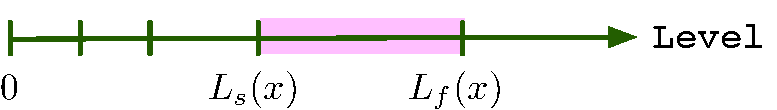
\includegraphics[width=3.5in]{home-stretch.pdf}
\end{center}
\caption{The tentative label $\yh_\ell(x)$ of a given point $x$ can undergo several mind-changes as the neighborhood of $x$ is sampled at successively higher levels. Between levels $L_s(x)$ and $L_f(x)$ there are contradicting labels on $x$, i.e.  $\yh_\ell(x)=!$. Beyond level $L_f(x)$, the correct label will be assigned.}
\label{fig:two-levels}
\end{figure}

We begin with $L_s$.

\begin{defn}
Pick any $x \in X$ with $\eta(x) \neq 0$ and let $s = \sign(\eta(x))$ be its Bayes-optimal label. We say $x$ is \emph{obscured} at level $\ell \geq 0$ if the following two conditions hold.
\begin{itemize}
\item No $B \in \B_\ell(x)$ has bias $s \cdot \eta_X(B) > b_2$.
\item Some $B \in \B_\ell(x)$ has bias $s \cdot \eta_X(B) < -b_1$.
\end{itemize}
Let $L_s(x)$ denote the smallest integer such that $x$ is not obscured at any level $\ell \geq L_s(x)$. If there is no such level, we define $L_s(x) = \infty$.
\label{defn:Ls}
\end{defn}
In words, for levels $\ell < L_s(x)$, there is no ball $B \in \B_\ell(x)$ which has a strong bias towards the correct (Bayes-optimal) label, and there are balls with at least a mild bias towards the wrong label.

Next, we define the level by which the label of a point ought to be apparent.
\begin{defn}
Pick any $x \in X$ with $\eta(x) \neq 0$ and let $s = \sign(\eta(x))$ be its Bayes-optimal label. We say $x$ is \emph{resolved} at level $\ell \geq 0$ if the following two conditions hold for all $\ell' \geq \ell$.
\begin{itemize}
\item All $B \in \B_{\ell'}(x)$ have $s \cdot \eta_X(B) > -b_1$.
\item Some $B \in \B_{\ell'}(x)$ has $s \cdot \eta_X(B) > b_2$.
\end{itemize}
Let $R_\ell$ denote the points that are resolved by level $\ell$. Let $L_f(x)$ denote the smallest level at which $x$ is resolved, or $\infty$ is there is no such level.
\label{defn:Lf}
\end{defn}
In words, for levels $\ell \geq L_f(x)$, no ball $B \in \B_\ell(x)$ has a strong bias towards the wrong label, and at least one ball has a strong bias towards the correct label.


Thus $L_s(x) \leq L_f(x)$, and there might be a large gap between the two. Before the background sampling reaches level $L_s(x)$, it is quite possible that we will predict the wrong label for $x$. However, once all balls in $\B_{L_s(x)}(x)$ have been adequately sampled, point $x$ will either (i) be assigned label $0$ or $!$, and put in the uncertainty set, in which case it will benefit from focused sampling, or (ii) will get the correct label. Once the balls in $\B_{L_f(x)}(x)$ have been sampled, condition (ii) will hold.

We define the set $F_\ell$ or include all of the points $x \in X$ such that $L_s(x) \leq \ell \leq L_f(x)$. The probability of $F_\ell$ determines the sample complexity of the active learning algorithm

\subsection{A possible characterization of $L_f(x),L_s(x)$}

\renewcommand{\P}{{\cal P}}
We are given a distribution over $\P$ over $\X \times \Y$ and a point $x \in X$.
We sample a set of unlabeled examples $X \subset \X$, and then run our active learning algorithm.

Our goal is to upper bound the number of samples $|\X|$ and the number
of queries the algorithm needs before the prediction of the algorithm
on $x$ converges to the correct label (and will not change with additional samples).

As we are dealing with the true distribution, we redifine $\B_\ell(x)$
to be all balls containing $x$ whose probability is in the range
$\left[ \frac{1}{2^{\ell-1}}, \frac{1}{2^\ell}\right]$.

Given the distribution $\P$, an edge parameter $\gamma>0$, a
prediction point $x$ and a level $\ell$ we partition the balls in $\B_{\ell}(x)$ into three 
subsets:
$$\B_{\ell}^+ = \{ B \in \B_\ell(x) | \eta(B)  > \gamma\},\;\;
\B_{\ell}^- = \{ B \in \B_\ell(x) | \eta(B)  < -\gamma\},\;\;
\B_{\ell}^0 = \{ B \in \B_\ell(x) | -\gamma \leq \eta(B) \leq \gamma\}$$

let the ``correct label'' of x be $s$, i.e. $s = \sign(\eta(x))$.
We define the ``true'' values of  $L_f(x),L_s(x)$ as follows:
\begin{itemize}
\item $L_s(x)$, is the smallest integer $m$ such that for all $\ell\geq
  m$, $\B_\ell^s \neq \emptyset$ while $\B_\ell^{-s} = \emptyset$.
\item $L_f(x)$ is the smallest integer $n \leq L_s(x)$ such that for
  all $n\leq \ell < L_s(x)$, $\B_\ell^s \neq \emptyset$ and $\B_\ell^{-s} \neq \emptyset$.
\end{itemize}

In other words the level $L_s(x)$ is the minimal level below which the
prediction is always correct. $L_f(x)$ is the minimal level above $L_s(x)$
such that the prediction on $x$ for the levels between  $L_f(x)$ and
$L_s(x)$ is always $!$.

\subsection{Another definition of two critical levels}
\yoav{I prefer to work with this definition}

For each point $x \in X$, we define two critical levels $L_0(x)$ and $L_1(x)$. 

Let $s = \mbox{sign}(\eta(x)) \in \{-1, +1\}$. Recall that $\PL_\ell(x) \subseteq \{-1,+1\}$ denotes the ``possible labels'' for $x$ after balls in $\B_\ell(x)$ have been queried.

We will define $L_0(x)$ and $L_1(x)$ so that: $s$ is guaranteed to be in $\PL_\ell(x)$ for all $\ell \geq L_0(x)$ and $-s$ is guaranteed to \emph{not} be in $\PL_\ell(x)$ for all $\ell \geq L_1(x)$. More precisely:
\begin{itemize}
\item $L_0(x)$ is the smallest level $\ell$ such that for all $\ell' \geq \ell$,
\begin{itemize}
\item there is a ball $B \in \B_{\ell'}(x)$ with $s \cdot \eta_X(B) > b_2$, and
\item any ball $B' \in \B_{\ell'}(x)$ with $B' \subset B$ has $s \cdot \eta_X(B') > -b_1$.
\end{itemize}
\item $L_1(x)$ is the smallest level $\ell$ such that for all $\ell' \geq \ell$, any ball $B \in \B_{\ell'}(x)$ either has $s \cdot \eta_X(B) > -b_1$ or contains some $B' \in \B_{\ell'}(x)$ with $s \cdot \eta_X(B') > b_2$.
\item \yoav{I would leave the definition of $L_0$ unchanged, but define $L_1$ as follows} $L_1(x)$ is the smallest level $\ell$ such that for all $L_0(x) > \ell' \geq \ell$, 
there exists two balls $B^+,B^- \in \B_{\ell'}(x)$ such that $\eta_X(B^+) > b_2$ and $\eta_X(B^-) < -b_2$.
\end{itemize}

Without containment:
\begin{itemize}
\item $L_0(x)$ is the smallest level $\ell$ such that for all $\ell' \geq \ell$, there is a ball $B \in \B_{\ell'}(x)$ with $s \cdot \eta_X(B) > b_2$.
\item $L_1(x)$ is the smallest level $\ell$ such that for all $\ell' \geq \ell$, there is no ball $B \in \B_{\ell'}(x)$ with $s \cdot \eta_X(B) < -b_1$.
\end{itemize}


\section{Characterizing $S_L,S_F$  for Euclidean balls}
Suppose the input
distribution is uniform on a ball $B$ of radius one  around the
origin. Denote the ``positive'' set to be $C$. Let $\gamma>0$ be the
edge such that
\[
  P(y=1|X=x) =\begin{cases}
    1/2+\gamma & \mbox{ if } x \in C \\
    1/2-\gamma & \mbox{ if } x \notin C
    \end{cases}
  \]

  $L_f(x)$ corresponds to half the distance between $x$ and the boundary

  $L_s(x)$ can be bounded independently of $x$ if $r$ is the largest
  radius such that both $C$ and $C^c$ can be expressed as a union of
  balls of radius $r$.

  We can define a bondary of bounded convexity in this way.


 For other definitions of ``ball'' we can use a similar
 characterization: $L_s(x)$ corresponds to the smallest ball
 containing both $x$ and a point with the opposite label. $L_f(x)$
 corresponds to the largest radius such that both $C$ and $C^c$ can be
 written as a union of balls.
  
\section{Examples}
\begin{itemize}
    \item 1D
    \begin{itemize}
        \item Single threshold with jump in $\eta$ ($-c$ on one side, $+c$ on the other side)
        \item Single threshold with more general $\eta$, e.g. Tsybakov condition
        \item Multiple thresholds with $-c, +c$
    \end{itemize}
    \item 2D all Euclidean balls
    \begin{itemize}
        \item Linear separator with $-c, +c$, e.g. uniform distribution over $x$\\
        I this case $L_s(x)$ is lower bounded the the probability of a
        ball whose radius is half the distance between $x$ and the
        linear separator. $L_f(x)$ is close to 0. Two large balls, one
        shifted towards the positive, the other shifted towards the
        negative, will suffice to create a disagreement.

        \item Separator of bounded curvature on both sides
    \end{itemize}
    \item Dyadic tree: instead of limiting attention to boxes that are cells of the tree, we look at all boxes of all sizes that supported on the underlying gridding of space. We get better bounds for two reasons:
    \begin{itemize}
        \item We look at large boxes, not just leaves of the tree.
        \item We use all boxes, not just those that are nested like the tree; this makes the boundary apparent earlier using !.
    \end{itemize}
    \item Arbitrary dimension, but Holder-smoothness and Tsybakov margin conditions (usual setting in nonparametric estimation). The rates obtainable using passive random sampling were determined by Audibert-Tsybakov. For active, can look at Hanneke. Will find out.
    \item A one-dimensional example, e.g. with data points in [0,1] and with
$\eta > 3/4$ or $\eta < 1/4$ everywhere. In this case, the balls could
be all intervals, or perhaps a finite collection of them based on some
gridding of the line. The Bayes-optimal classifier would have a finite
number of sign-changes, and we could quantify which of these we'd pick
up by each level of sampling.

\item A high-dimensional Euclidean setting in which we use balls
corresponding to the cells of a tree (e.g. RP tree).

\item A high-dimensional metric space setting in which we have a
collection of metric balls and we give label complexity bounds based
on smoothness conditions (Holder-smoothness of the $\eta$ function)
and boundary conditions (like Tsybakov margin condition).

\end{itemize}


\begin{figure}
\begin{center}
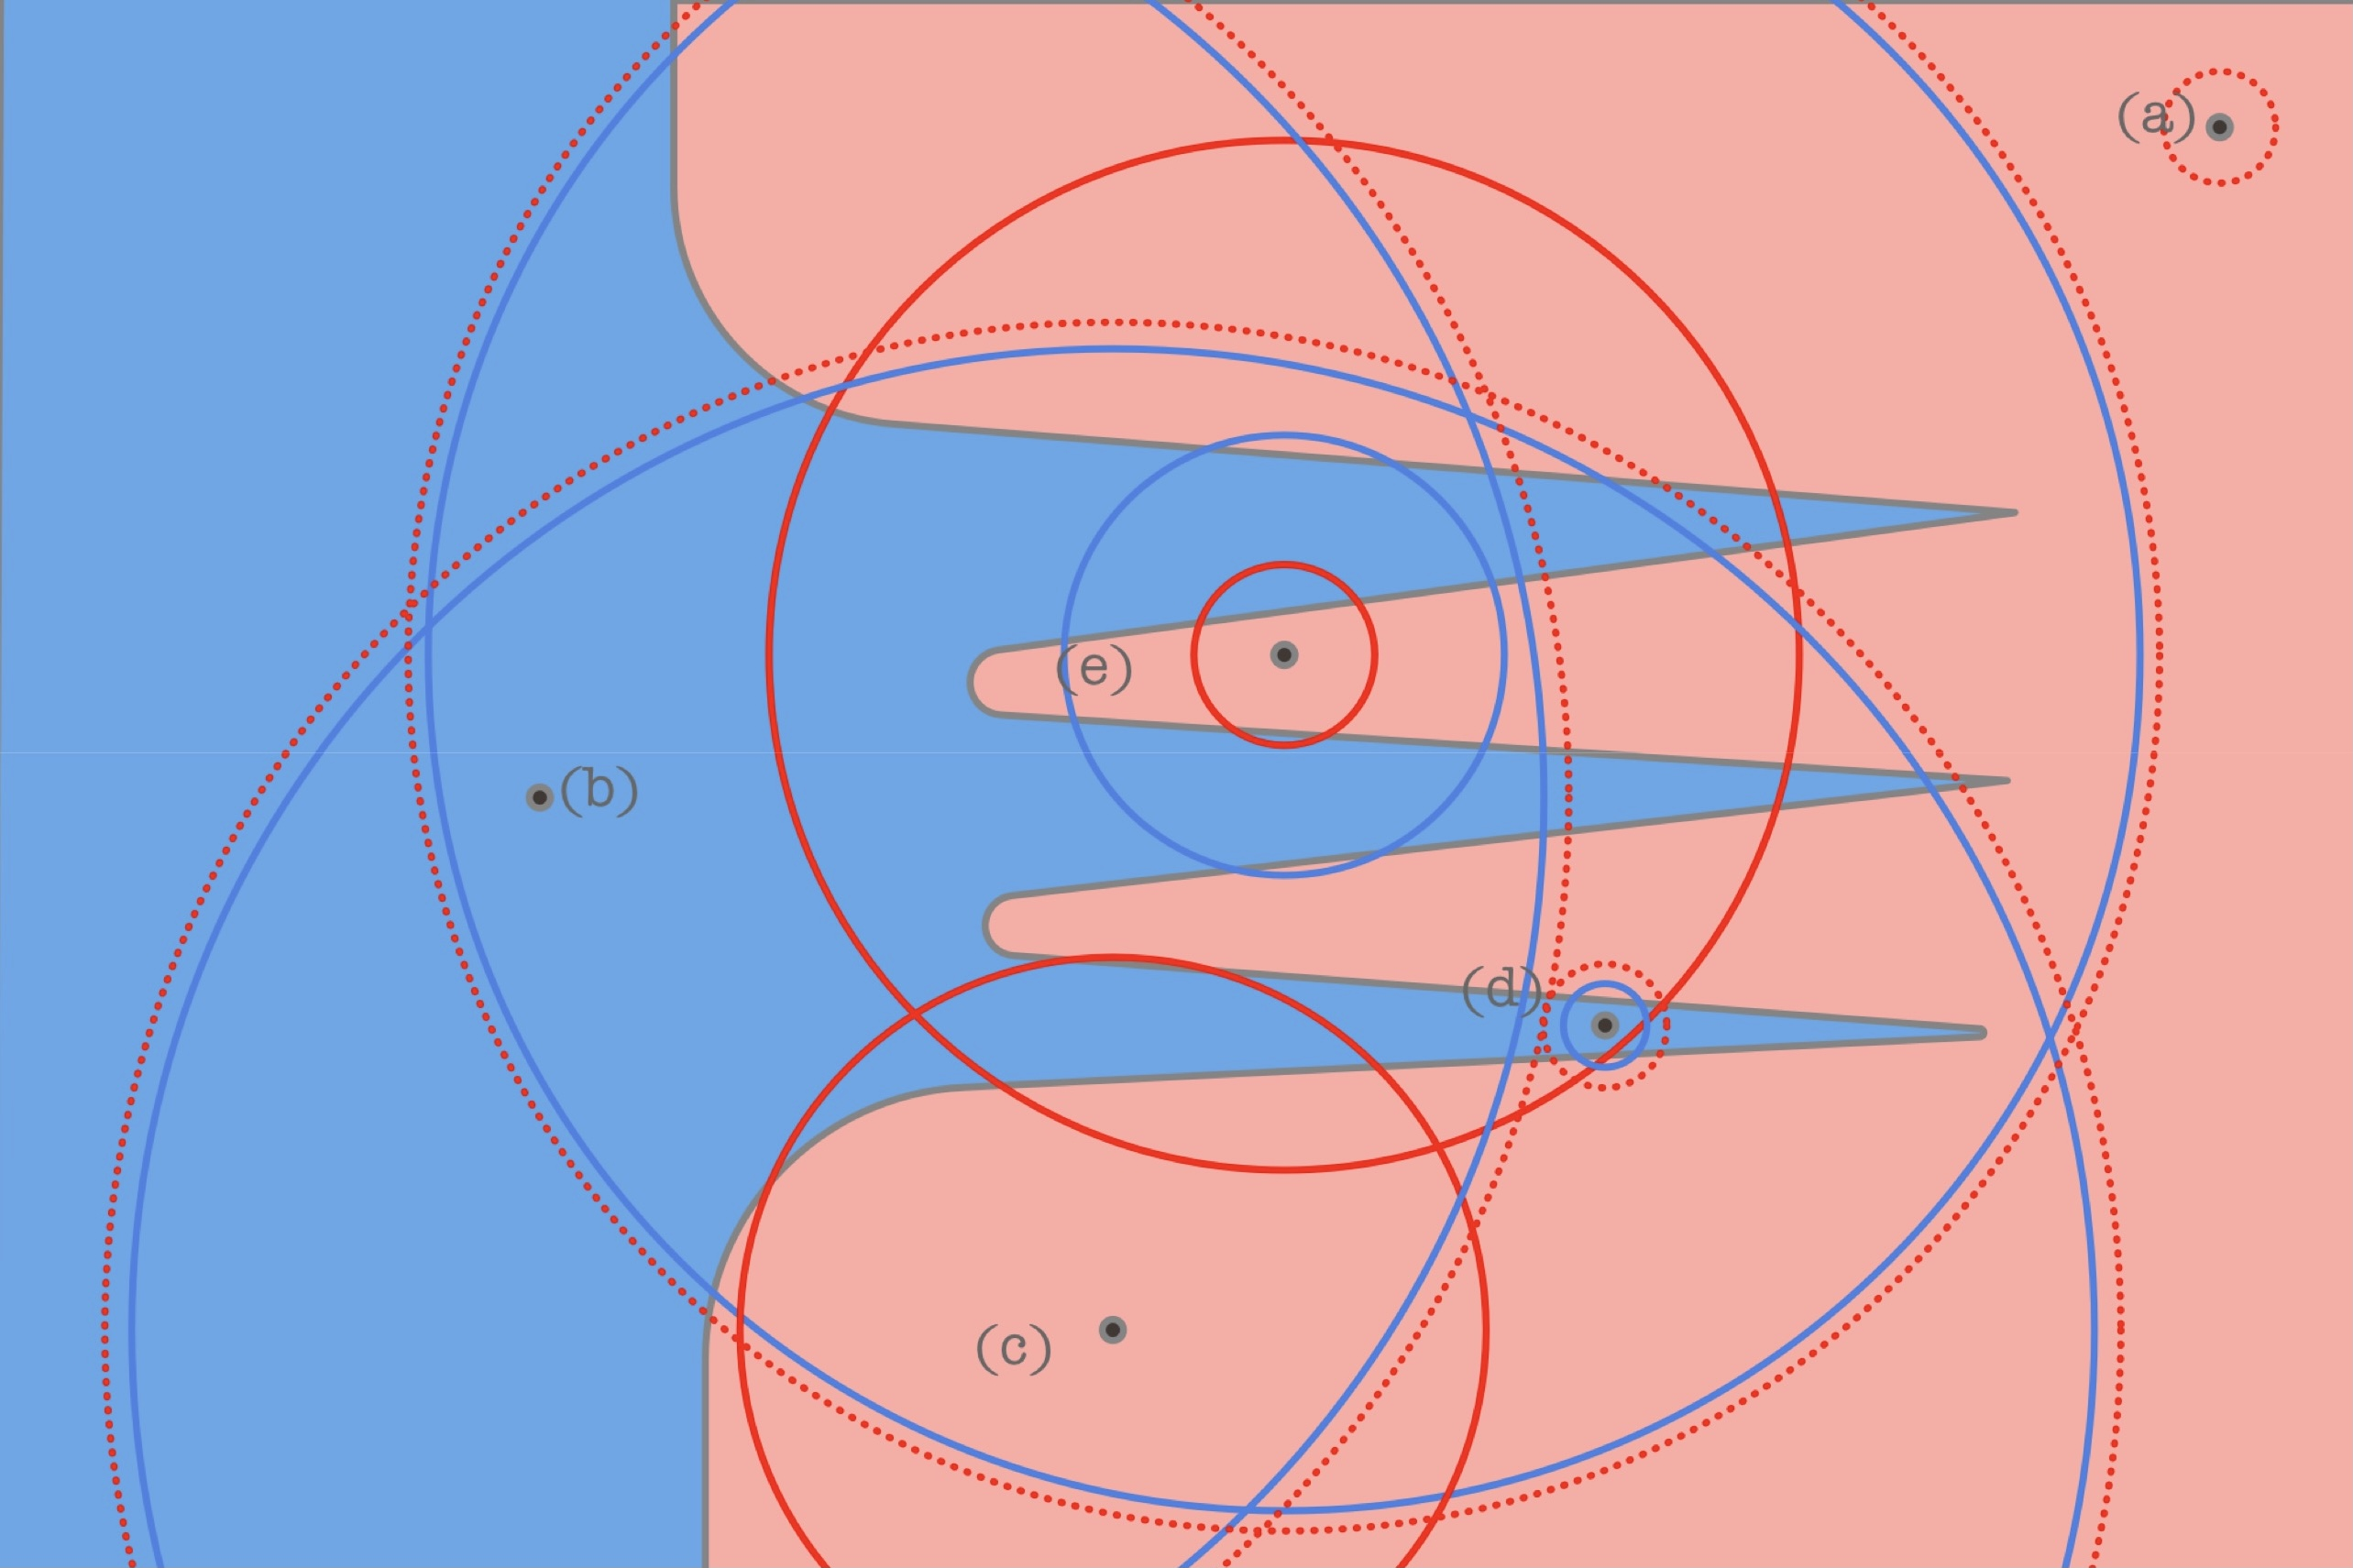
\includegraphics[width=6in]{IMG_0840.jpg}
\end{center}

\caption{\yoav{Picture should be changed to include circles containing $x$ but not centered at $x$.} This figure provides some examples for the concept of mind changes. Here we consider true probabilities, rather than estimates. The bounding rectangle defines the input space $X$. The blue region indicate $x$'s where the probability of +1 is larger than that of $-1$, the red region indicates the revers polarity. More specifically, we assume that in the blue region the probability of +1 is 0.6, while in the red region the probability of +1 is 0.4.
The black dots correspond to points on which we want to make a prediction. We consider all circles centered at each point. The {\em bias} of  circle is the probability of +1 conditioned on the point being in the circle. As labels are accumulated, the bias of smaller and smaller circles can be determined. For any point there is a large enough circle that contains the whole input space. We assume that the overall bias is negative, hence for a sufficiently large circle the bias is negative. This is indicated by the dotted circle which is always the largest circle. The solid line circles are the largest circles with the polarity indicated by the color of the line. The smallest circle corresponds to the last mind change which we also call the convergence circle.
A point is considered "easy" if its convergence circle is large, because that means that a small number of queries is required to find the correct label.
Following that definition we get that the order of points from the easiest to the hardest is {\bf a,b,c,e,d}. Comparing e and d we see that d has a smaller convergence circle, and one mind change, which (e) has a larger convergence circle, but has 4 mind changes.
}

\label{fig:mind-changes}
\end{figure}

\pagebreak

\section{Technicalities}

\subsection{Large deviation bounds}

\begin{lemma}
Fix a confidence parameter $0 < \delta < 1$ and a positive integer $k \geq 6 \ln (4/\delta)$. 

Let $x_1, \ldots, x_m$ be any collection of points. Suppose that the labels $Y_i \in \{-1,1\}$ of these points are independent, with $\E Y_i = \eta(x_i)$. Define
$$ \eta_o = \frac{1}{m} \left( \eta(x_1) + \cdots + \eta(x_m) \right) .$$
Now consider the following estimator $Z$ of this quantity:
\begin{itemize}
\item Each $x_i$ is chosen with probability $q > 0$, independently. Let $N$ be the number of selected points.
\item If $N > 0$, the labels $Y_i$ of the selected points are obtained, and $Z$ is their average.
\end{itemize}
If $qm \geq k + \sqrt{6k \ln (4/\delta)}$, with probability at least $1-\delta$, 
\begin{enumerate}
\item[(a)] $N \geq k$, and 
\item[(b)] $| Z - \eta_o| \leq \sqrt{(48/k) \ln (4/\delta)}$.
\end{enumerate}
\label{lemma:large-deviation-discrete}
\end{lemma}
\begin{proof}
Let's start with (a). Define $c_1 = \sqrt{3 \ln (4/\delta)}$. We'll take $qm = k + \sqrt{6k \ln (4/\delta)} = k + c_1 \sqrt{2k}$ since this is the worst case. By assumption, $k \geq 2c_1^2$ and thus $qm \leq 2k$.

Now, $N$ has a binomial($m,q$) distribution. By a multiplicative Chernoff bound, for $0 < \epsilon < 1$, we have
\begin{align*}
\pr(N \geq qm(1+\epsilon)) &\leq e^{-qm\epsilon^2/3} \\
\pr(N \leq qm(1-\epsilon)) &\leq e^{-qm\epsilon^2/2}
\end{align*}
Take $\epsilon = c_1/\sqrt{qm}$; by the lower bound on $k$, we have $\epsilon \leq 1/2$. Recalling the choice of $c_1$, we see that with probability at least $1-\delta/2$, we get 
$$(1-\epsilon) qm < N < (1+\epsilon) qm .$$
The lower bound implies $N > qm(1-\epsilon) = qm - c_1\sqrt{qm} = k + c_1 \sqrt{2k} - c_1 \sqrt{qm} \geq k$.

For (b), define $C_1, \ldots, C_m \in \{0,1\}$ as random variables indicating whether the corresponding points were selected; that is, $C_i = {\bf 1}(\mbox{$x_i$ was selected})$. The sum of the obtained labels is then $S = C_1 Y_1 + \cdots + C_m Y_m$. Notice that these $C_iY_i \in \{-1,0,1\}$ are independent with $\E[C_iY_i] = q \eta(x_i)$ and $\E[(C_iY_i)^2] = \E[C_i] = q$. Thus their sum $S$ has expectation
$$ \E [S] = \sum_{i=1}^m \E[C_i Y_i] = \sum_{i=1}^m q \eta(x_i) = qm \eta_o $$
and variance
$$ \mbox{var}(S) = \sum_{i=1}^m \mbox{var}(C_iY_i) \leq qm .$$
We can bound the concentration of $S$ around its expected value using Bernstein's inequality, by which
$$ \pr(|S - \E[S]| \geq t) \leq 2 \exp \left( - \frac{t^2}{2(\mbox{var}(S) + 2t/3)} \right) .$$
Using $t = \epsilon qm$, we then have that $|S - qm \eta_o| \leq \epsilon qm$ with probability at least $1-\delta/2$.

Combining with the high-probability bound on $N$ above, we get
$$ \frac{qm \eta_o - \epsilon qm}{qm(1+\epsilon)} < \frac{S}{N} < \frac{qm \eta_o + \epsilon qm}{qm(1-\epsilon)},$$
whereupon (recalling $Z = S/N$)
$$ 
\eta_o \left( \frac{1}{1+\epsilon} -1 \right) - \frac{\epsilon}{1+\epsilon} < Z - \eta_o < \eta_o \left( \frac{1}{1-\epsilon} - 1 \right) + \frac{\epsilon}{1-\epsilon} .$$
Since $|\eta_o| \leq 1$,
$$ |Z - \eta_o | \leq \max \left( \frac{2\epsilon}{1+\epsilon}, \frac{2\epsilon}{1-\epsilon} \right)
\leq 
4 \epsilon,$$
as claimed.  
\end{proof}


\end{document}

